\documentclass[a4paper,12pt]{article}

\title{Laba}
\author{Георгий Демьянов}
\date{today}
\usepackage[T2A]{fontenc}
\usepackage[utf8]{inputenc}
\usepackage[english,russian]{babel}
\usepackage{amsmath,amsfonts,amssymb,amsthm,mathtools,bpchem}
\usepackage{fancyhdr}
\usepackage{indentfirst}
\usepackage{float}
\usepackage{etaremune}

\usepackage[margin=1in]{geometry}

\pagestyle{fancy}
\fancyhf{}
\rhead{\thepage}
\renewcommand{\headrulewidth}{0pt}

\thispagestyle{empty}


\begin{document}
\begin{titlepage}
\begin{center} 
 
\large Московский физико-технический институт\\
Факультет молекулярной и химической физики\\
\vspace{7cm}
\Large Лабораторная работа \\по курсу \\ Физические методы исследований\\
\textbf{\Large <<ИЗМЕРЕНИЕ ВРАЩАТЕЛЬНОЙ И КОЛЕБАТЕЛЬНОЙ ТЕМПЕРАТУР В ГАЗОВОМ РАЗРЯДЕ ПО СПЕКТРУ МОЛЕКУЛЫ $N_2$ >>}\\
\end{center} 

\vspace{5cm}
{\par 
	\raggedleft \large 
	\emph{Выполнили:}\\ 
	студенты 3 курса\\ 
	643 группы ФМХФ\\ 
	Зарубин Всеволод  \\ 
	Мишина Аня 
\par}
\begin{center}
\vfill \today
\end{center}
\end{titlepage}
\newpage
\setcounter{page}{2}

\newpage
	\section{Постановка задачи}
	В данной работе необходимо было определить вращательную температуру в газоразрядной воздушной плазме по неразрешенной вращательной структуре
излучения 0–0- полосы (2+)-системы азота и колебательную температуру по относительной интенсивности
электронно-колебательных полос (2+)-системы азота. Также провести идентификацию наблюдаемых в спектрах полос. 
	\section{Теоретические сведения}
	
	\subsection{Молекулярные спектры, правила отбора}
	
	В отличие от атомов, у которых каждому электронному состоянию соответствует
уровень энергии, имеющий определенное значение, об энергии молекул можно говорить лишь при фиксации положения ядер. Поэтому уровни энергии молекулы или, как их называют, электронные термы, представляют собой функции от взаимного расположения
ядер. В простейшем случае двухатомной молекулы электронный терм является функцией
энергии молекулы от расстояния между ядрами. Полное энергетическое состояние молекулы зависит также от ее колебательного и
вращательного движений. Энергии этих степеней свободы имеют дискретные значения и
описываются колебательным квантовым числом ($\nu$) и полным вращательным квантовым
числом ($J$). Рассмотрим теперь переходы между различными состояниями молекулы.
Переходы с изменением только вращательного числа называются вращательными, с
изменением колебательного числа — колебательно-вращательными, с изменением
электронного состояния — электронно-колебательно-вращательными. В дальнейшем будем
говорить об электронно-колебательно-вращательных переходах. Допустимые переходы между различными электронными состояниями подчинены некоторым правилам отбора.
Эти правила зависят от типа связи между орбитальным движением электронов, их спином
и вращением молекулы. Во многих важных случаях правила отбора следующие:
	
\begin{enumerate}
	
	\item $\Delta \Lambda = 0, \pm 1 $ , 
	\item мультиплетность $2S+1$ не меняется,
	\item соблюдение принципа Франка-Кондона,
	\item при изменении вращательного квантового числа $\Delta J = 0, \pm 1 $, причем запрещен переход 0~$\rightarrow $~0,
	\item для перехода $ \Sigma \rightarrow \Sigma $ выполняется $ \Delta J \neq 0$.	
\end{enumerate}

	
	\subsection{ Методы измерения $T_rot$ , $T_vib$}
	 
	Для измерения вращательной температуры необходимо получить спектр 0 $\rightarrow $ 0 полосы ($2^+$)-системы молекулы азота в режиме неразрешенной вращательной структуры. После получения спектра необходимо найти десятичный логарифм от интенсивностей и построить график зависимости lgI от $\lambda$, выделить прямолинейный участок, найти тангенс угла наклона прямой и по рисунку определить значение вращательной температуры.
	\begin{figure}[h]
		\begin{center}
			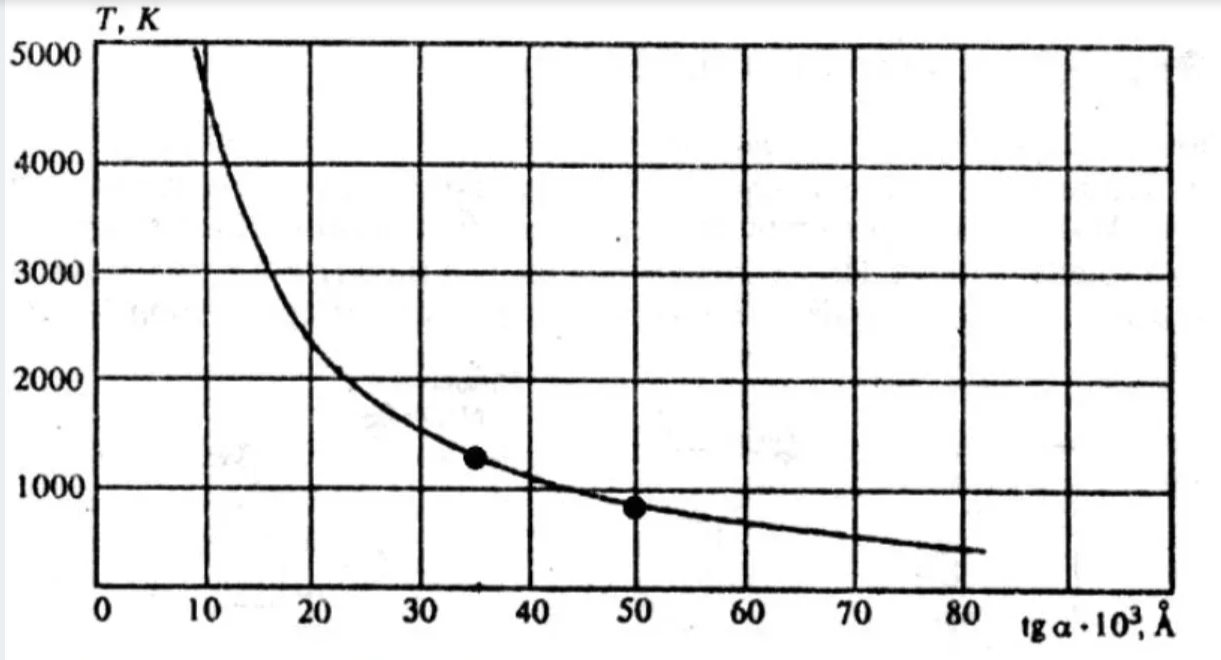
\includegraphics[scale=0.5]{kalibr}
			\caption{Каллибровочная кривая}
		\end{center}
	\end{figure}
Для измерения колебательной температуры необходимо записать спектры полос 0 $\rightarrow $ 1, 1 $\rightarrow $ 2, 0 $\rightarrow $ 2, 1 $\rightarrow $ 3 ($2^{+}$)-системы. Далее по формуле 3 определяем вращательную температуру.

	\section{Описание установки}
	В данной работе источником излучения служит тлеющий разряд в воздухе.
Принципиальная схема регистрации излучения на схеме ниже. Излучение
регистрируется через боковую стенку разрядного отсека плазмотрона. Изображение плазмы в
масштабе 1:4 с помощью линзы из LiF фокусируется на входную щель монохроматора МДР-23.

	\begin{figure}[h]
		\begin{center}
			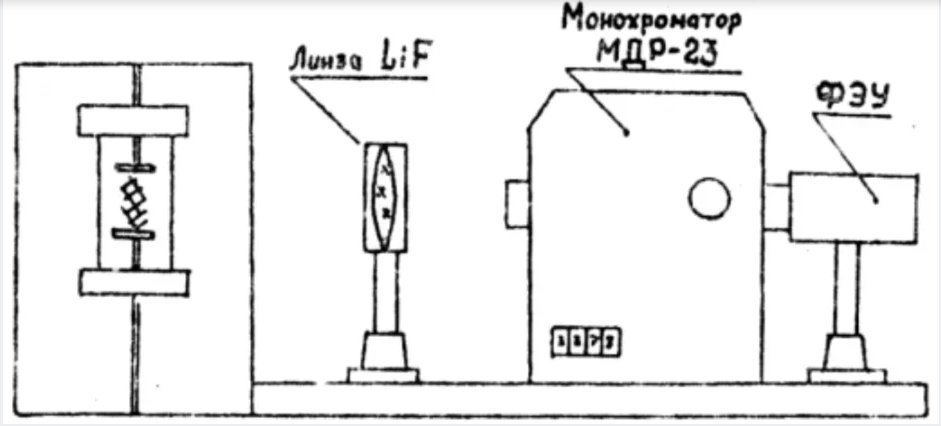
\includegraphics[scale=0.5]{ystanovka}
			\caption{Схема установки}
		\end{center}
	\end{figure}

В качестве диспергирующего элемента монохроматора используется дифракционная
решетка, имеющая 1200 штрихов на миллиметр (1200 /1). За выходной щелью
монохроматора помешается фотоумножитель ФЭУ-100. Монохроматор МДР-23
используется в составе управляющего измерительного комплекса КСВУ-23, включающего
также ЭВМ ДВК-3, интерфейсные блоки связи ЭВМ с экспериментальной установкой,
усилитель с высокоомным входом, управляемый от ЭВМ источник высокого напряжения
для питания ФЭУ. Конструкция монохроматора позволяет осуществлять сканирование
спектра в автоматическом режиме с заданной скоростью. Дифракционная решетка при
этом поворачивается с помощью шагового двигателя.


Использование воздушной смеси азота и кислорода принципиально, так как при содержании кислорода менее 2 \% в спектре появляются полосы отрицательной ($1^{-}$)-системы ${N_2}^+$, чья интенивность может превосходить интенсивность (2+) системы.  


\newpage
	
	\section{Экспериментальная часть}
	
	\subsection{Спектры (2+)-системы при разных значения давления}
	
	\begin{figure}[h]
	\begin{center}
	\begin{minipage}[h]{0.45\linewidth}
	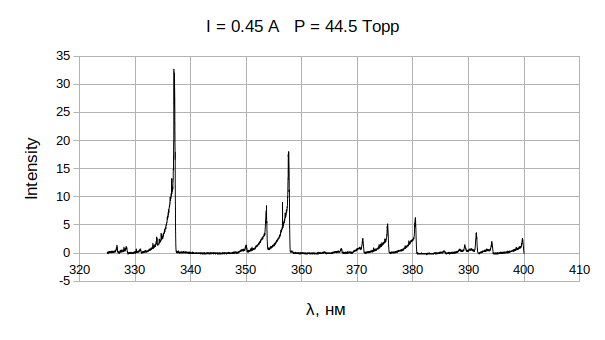
\includegraphics[width=1\linewidth]{44_5_full}
	\caption{P = 44.5 Торр, I = 0.45 A} %% подпись к рисунку
	\end{minipage}
	\hfill
	\begin{minipage}[h]{0.45\linewidth}
	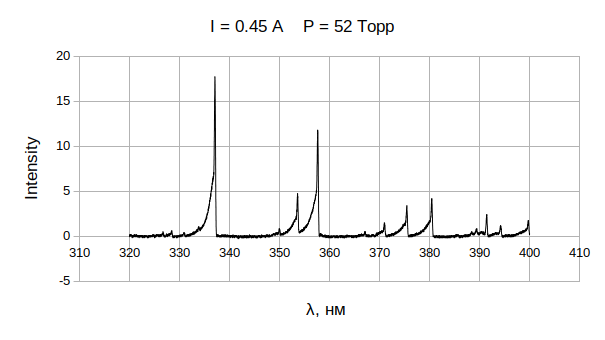
\includegraphics[width=1\linewidth]{52_full}
	\caption{P = 52 Торр, I = 0.45 A}
	\end{minipage}
	\end{center}
	\end{figure}
	
	\begin{figure}[h]
	\begin{center}
	\begin{minipage}[h]{0.45\linewidth}
	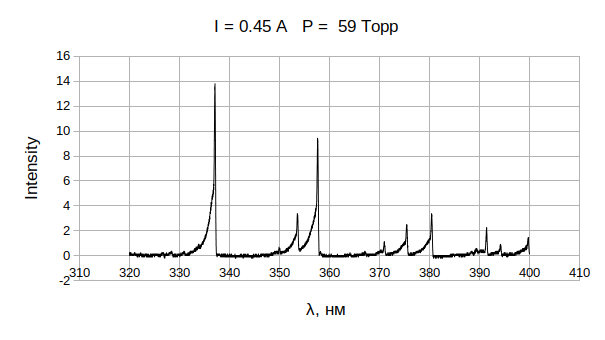
\includegraphics[width=1\linewidth]{59_full}
	\caption{P = 59 Торр, I = 0.45 A} %% подпись к рисунку
	\end{minipage}
	\hfill
	\begin{minipage}[h]{0.45\linewidth}
	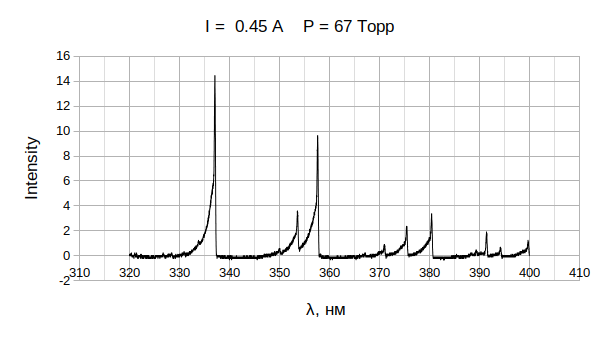
\includegraphics[width=1\linewidth]{67_full}
	\caption{P = 67 Торр, I = 0.45 A}
	\end{minipage}
	\end{center}
	\end{figure}
	
	\begin{figure}[h]
	\begin{center}
	\begin{minipage}[h]{0.45\linewidth}
	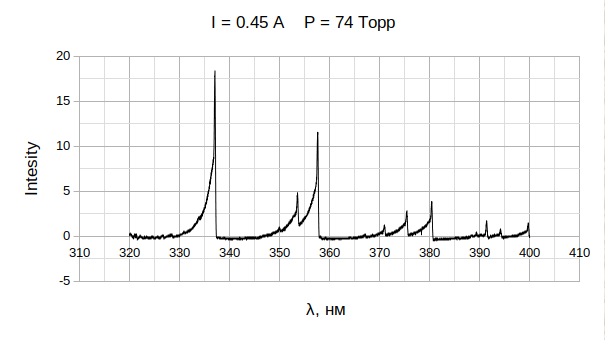
\includegraphics[width=1\linewidth]{74_full}
	\caption{P = 74 Торр, I = 0.45 A} %% подпись к рисунку
	\end{minipage}
	\hfill
	\end{center}
	\end{figure}
	
\newpage

	\subsection{Спектры (2+)-системы при разных значениях силы тока}
		\begin{figure}[H]
		\begin{center}
			\includegraphics[scale=0.3]{I_full}
			\caption{Спектры (2+)-системы при разнх значениях силы тока}
		\end{center}
	\end{figure}
	
\newpage
Произведем соотнесение полос наблюдаемых в полеченных спектрах.

	\begin{figure}[H]
		\begin{center}
			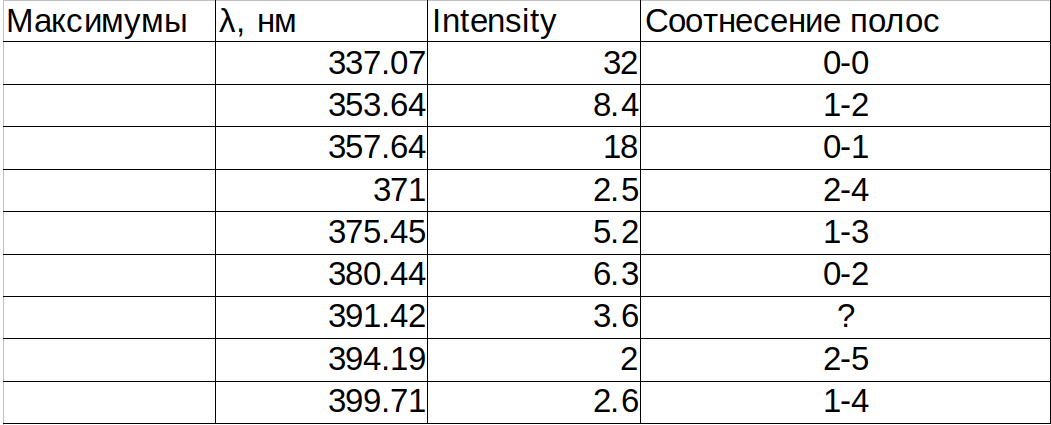
\includegraphics[scale=0.4]{polosi}
			\caption{Наблюдаемые в спектре полосы}
		\end{center}
	\end{figure}
	
\newpage
	\subsection{Определение $T_{rot}$ при разных значениях давления}
	Для вычисления вращательной температуры выберем участок неразрешенной
вращательной структуры и прологарифмируем его. По наклону прямой зависимости $\lg I=f(\lambda)$ , используя рассчитанную
зависимость тангенса угла наклона от значения вращательной температуры, определим значение вращательной температуры в центральной части
разряда.

	\begin{figure}[h]
	\begin{center}
	\begin{minipage}[h]{0.45\linewidth}
	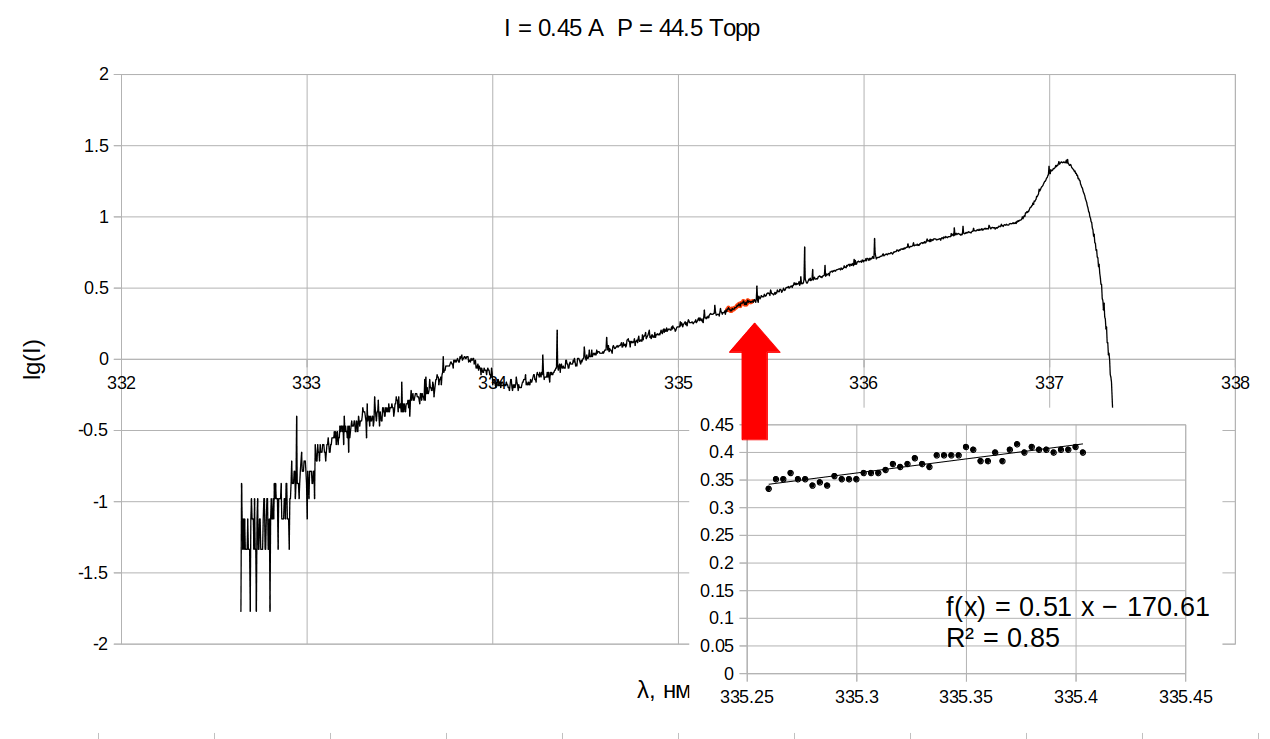
\includegraphics[width=1\linewidth]{p_44_5}
	\caption{P = 44.5 Торр, I = 0.45 A} %% подпись к рисунку
	\end{minipage}
	\hfill
	\begin{minipage}[h]{0.45\linewidth}
	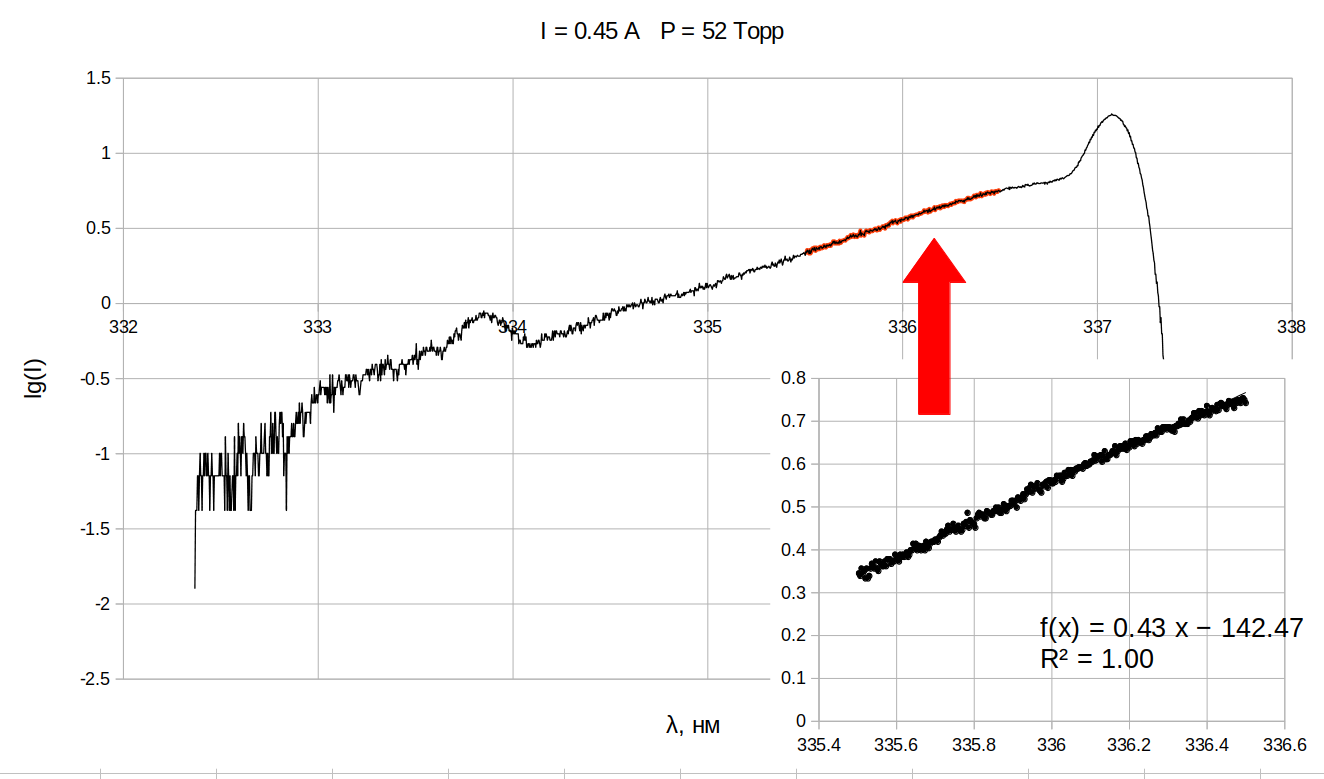
\includegraphics[width=1\linewidth]{p_52}
	\caption{P = 52 Торр, I = 0.45 A}
	\end{minipage}
	\end{center}
	\end{figure}
	
	\begin{figure}[h]
	\begin{center}
	\begin{minipage}[h]{0.45\linewidth}
	\includegraphics[width=1\linewidth]{P_59}
	\caption{P = 59 Торр, I = 0.45 A} %% подпись к рисунку
	\end{minipage}
	\hfill
	\begin{minipage}[h]{0.45\linewidth}
	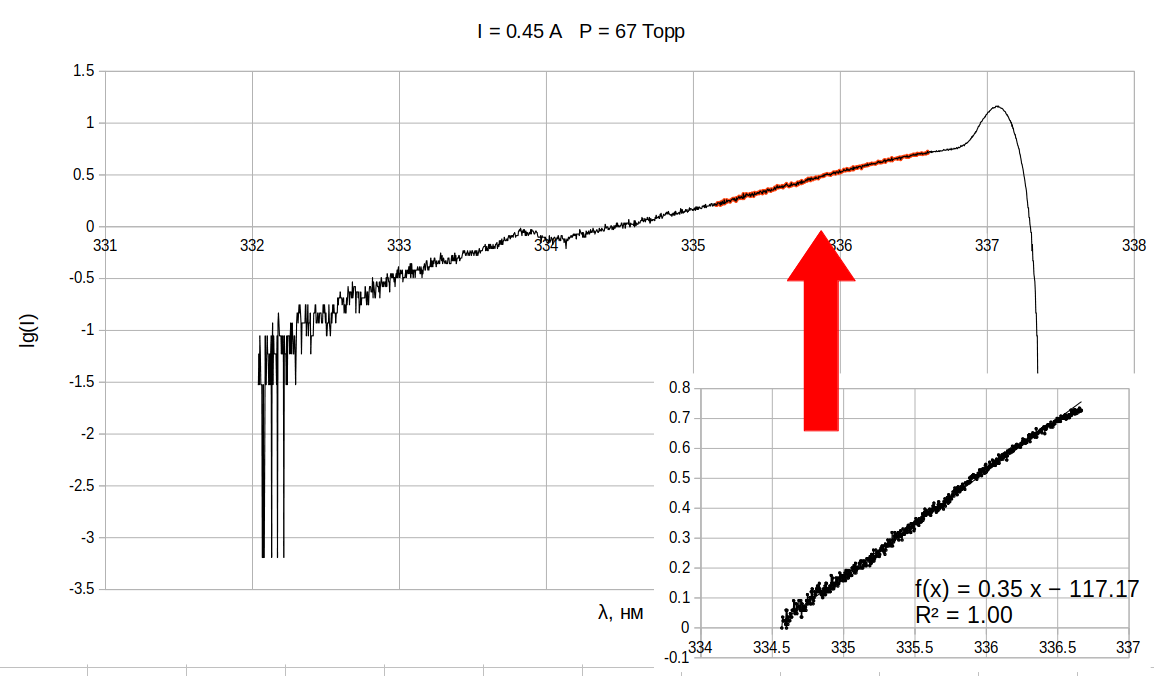
\includegraphics[width=1\linewidth]{p_67}
	\caption{P = 67 Торр, I = 0.45 A}
	\end{minipage}
	\end{center}
	\end{figure}
	
	\begin{figure}[h]
	\begin{center}
	\begin{minipage}[h]{0.45\linewidth}
	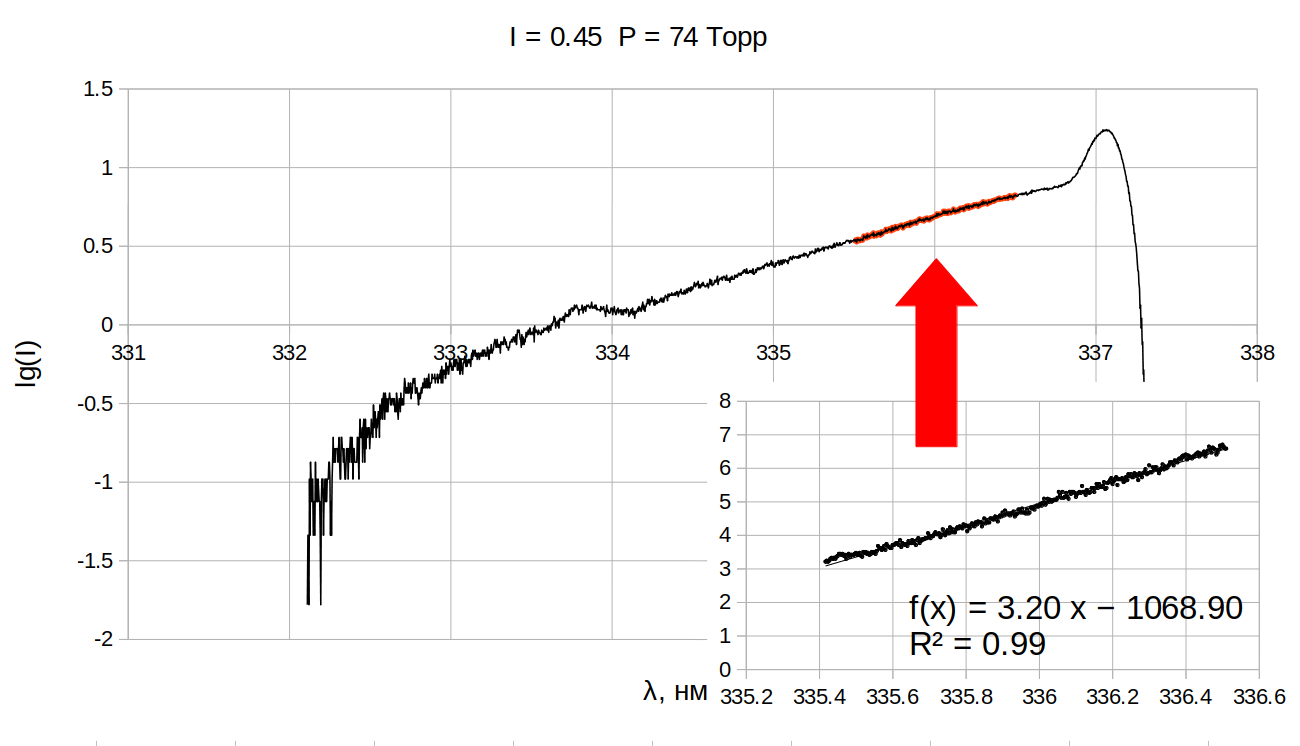
\includegraphics[width=1\linewidth]{p_74}
	\caption{P = 74 Торр, I = 0.45 A} %% подпись к рисунку
	\end{minipage}
	\hfill
	\end{center}
	\end{figure}
	
\newpage
По вычисленным коэффициентам наклона, используя калибровочную кривую (см. раздел Методы вычисления вращательных и колебательных температур) находим $T_{rot}$. 
	\begin{figure}[H]
		\begin{center}
			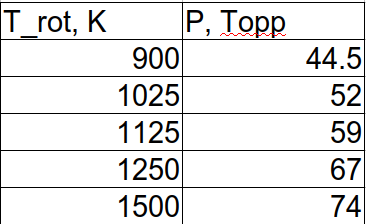
\includegraphics[scale=0.4]{rot_P}
			\caption{$T_{rot}$ при разных значения давления}
		\end{center}
	\end{figure}

\vspace{5cm}
	\subsection{Определение $T_{rot}$ при разных значениях силы тока}
	
\vspace{3cm}
     Сведем данные о вычисленных $T_{rot}$ в таблицу.
	\begin{figure}[H]
		\begin{center}
			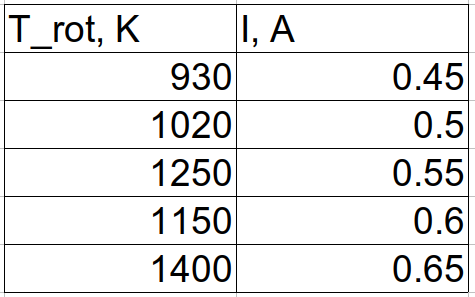
\includegraphics[scale=0.4]{rot_I}
			\caption{$T_{rot}$ при разных значения силы тока}
		\end{center}
	\end{figure}
	
\newpage    
	\begin{figure}[H]
		\begin{center}
			\includegraphics[scale=0.3]{log_I}
			\caption{Прологорифмированная интесивность в зависимости от длины волны при разных значениях силы тока}
		\end{center}
	\end{figure}
	
\newpage
	\begin{figure}[H]
		\begin{center}
			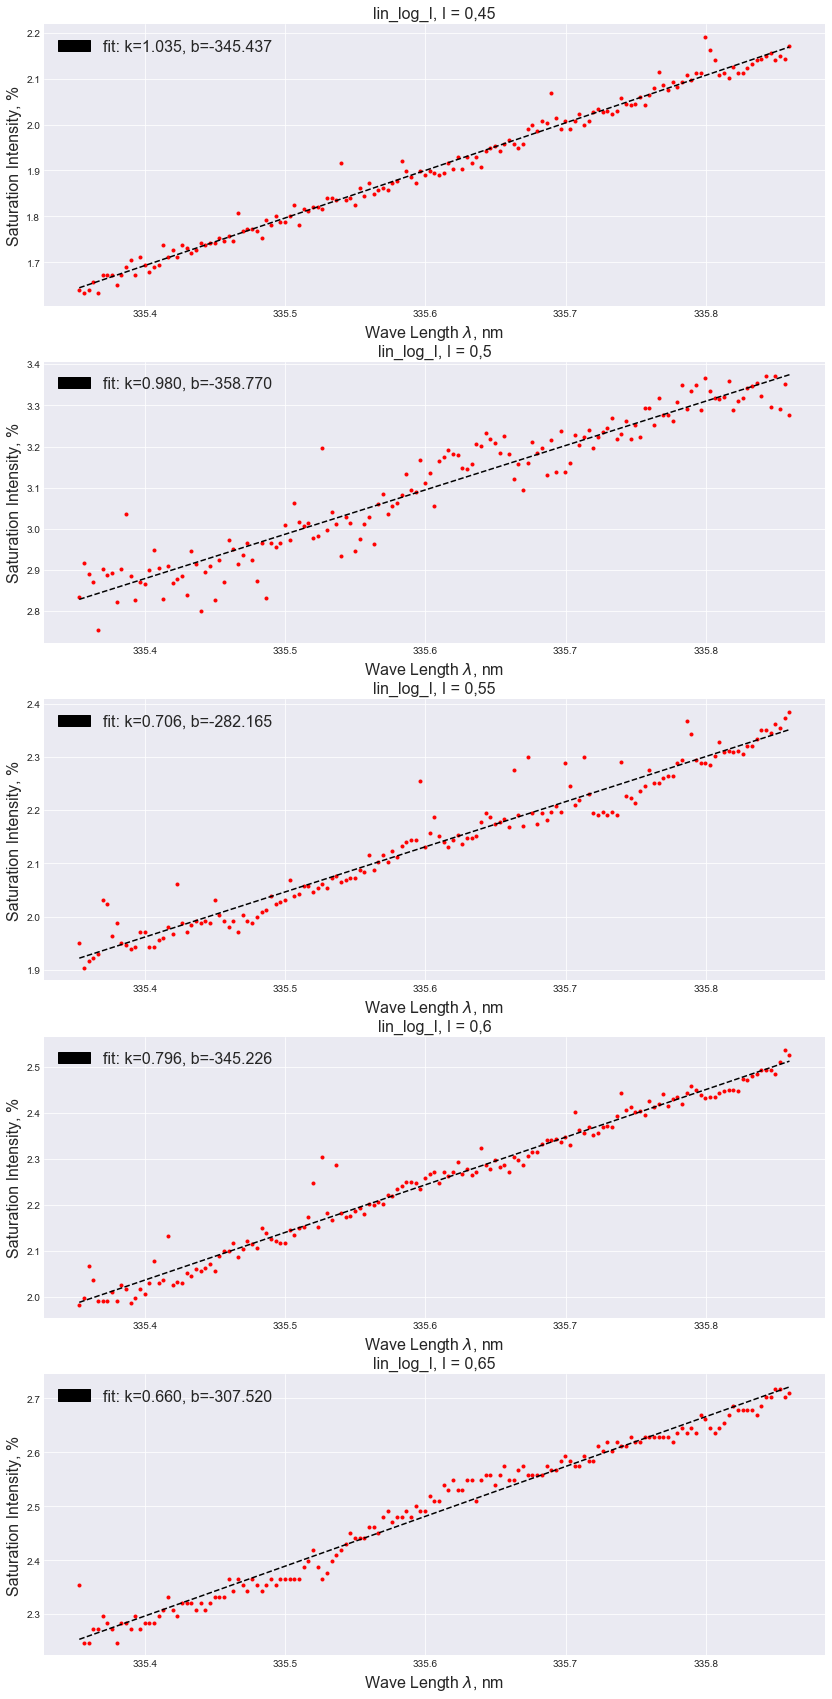
\includegraphics[scale=0.4]{dependence_of_I}
			\caption{Вспомогательные рисунки к вычислению $T_{rot}$}
		\end{center}
	\end{figure}
	
\newpage
	\begin{figure}[H]
		\begin{center}
			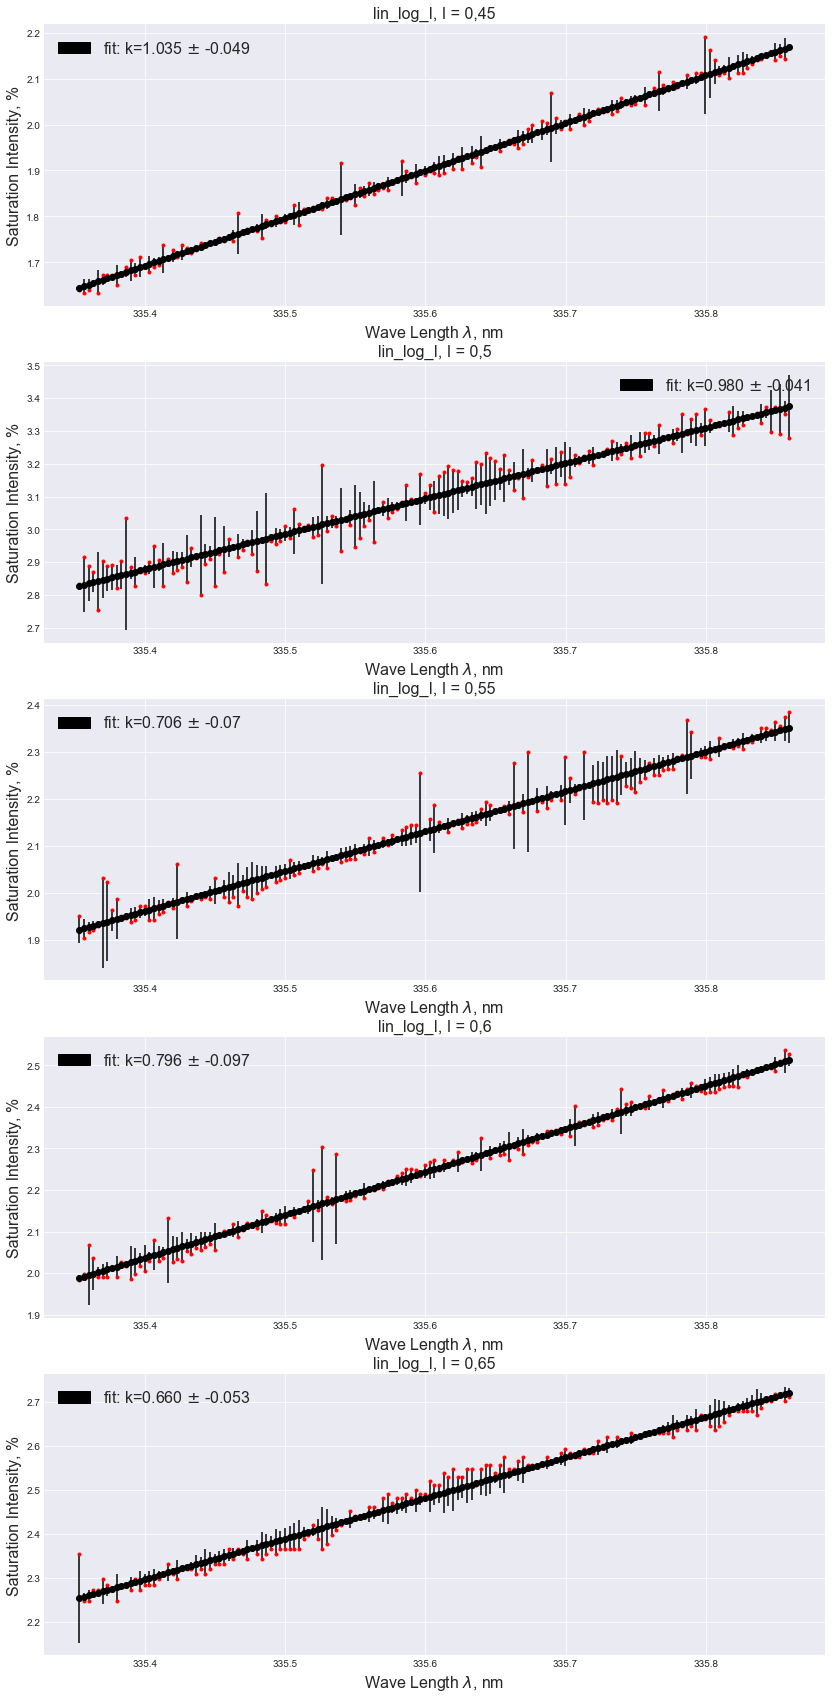
\includegraphics[scale=0.4]{I_dep_error}
			\caption{ Кресты ошибок}
		\end{center}
	\end{figure}
	
	
		

\newpage
	\subsection{Определение $T_{vib}$}
По спектрам полос $0\to1$, $1\to2$ , $2 \to3$ ; $0 \to 2$ ,$1\to 3$,$2 \to 4$ определим
колебательную температуру в центральной части разряда и в приэлектродных
областях, используя соотношение
\begin{equation}
\ln\cfrac{I_{v'v''}}{\nu^4_{v'v''}q_{v'v''}} = -\cfrac{G(v')}{0.6925 T_{vib}} +C.
\end{equation}
	

		\begin{center}
		 I = 0.45 A, p = 44.5 торр
		\end{center}       
		\begin{figure}[H]
		\begin{center}
			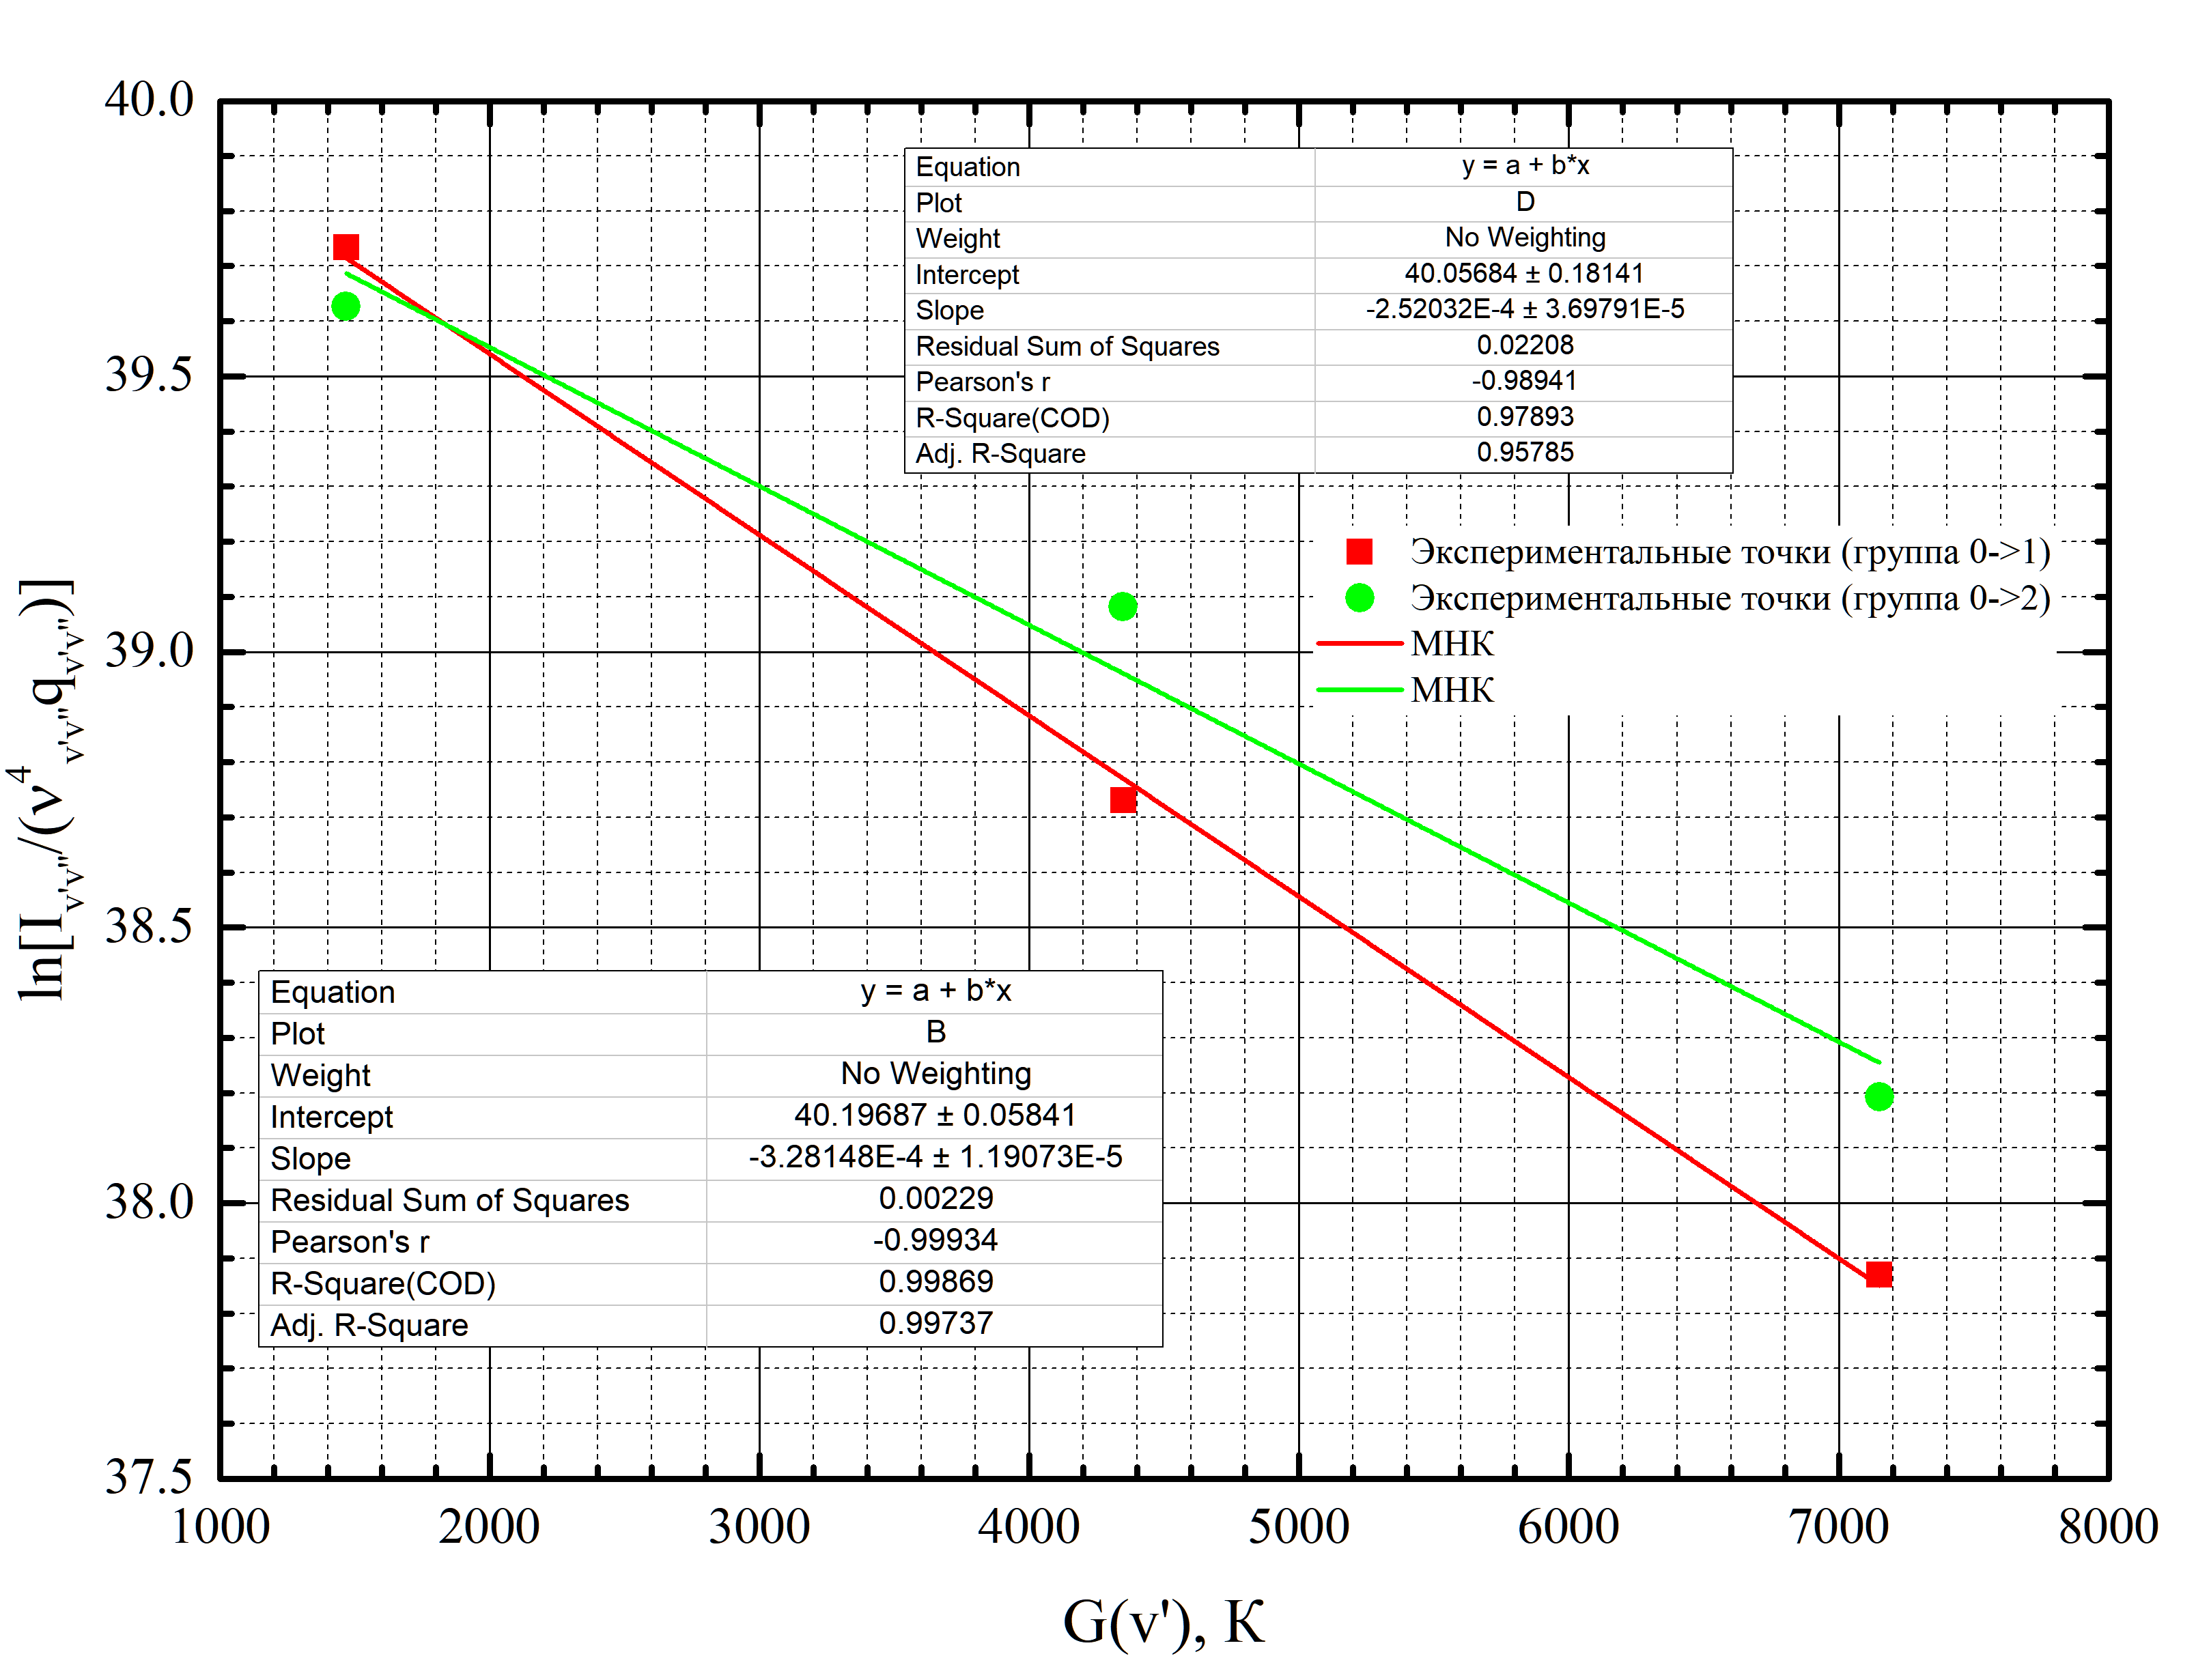
\includegraphics[scale=0.4]{vib}
			\caption{Определение $T_{vib}$}
		\end{center}
	\end{figure}
	
Результаты:
	\begin{eqnarray}
	T_{\text{колеб, 1}} = (3.5\pm0.2)\cdot10^3 \text{ К}\\
	T_{\text{колеб, 2}} = (4.1\pm0.5)\cdot10^3 \text{ К}
	\end{eqnarray}
	
	\section{Заключение}
	В данной работе были получены электронно-колебательно-вращательные спектры, качественный вид которых не изменялся в исследуемом диапазоне давлений (от 44.5 до 74 Торр) и токов (от
0.45 А до 0.65 А). Также были посчитаны вращательные температуры по электронно-колебательно-вращательным спектрам излучения второй положительной системы азота при разных токах и
давлениях, а так же колебательные температуры. Используемая методика нахождения этих температур даёт адекватные, но грубые результаты. Оказалось, что при повышении силы тока или
давления в газе вращательная температура увеличивается.
	

\end{document}
